\par Voir la section \ref{methodologie} et l'organigramme de la figure \ref{fig:methodologie1} pour la représentation graphique de la méthodologie, et dont les phases peuvent être résumées de la façon suivante:  
\begin{itemize}
   \item Recherche des références, des modèles et des données, ainsi que l'équipement pour le nano-ordinateur et des logiciels nécessaires.
   \item Installation sur le Jetson nano du système d'exploitation, de l'environnement de développement et de tests pour l'inférence.
   \item Itération entre les étapes suivantes:
   \begin{itemize}
      \item Inférence avec le Jetson nano en utilisant les modèles et les sources de données sélectionnées.
      \item Adaptation des modèles à différentes résolutions d'images et à la zone d'étude.
      \item Traitement des données afin de les adapter au requis des modèles.
   \end{itemize}
\end{itemize}

\label{methodologie}
L'organigramme de la figure \ref{fig:methodologie1} présente la démarche de la réalisation du projet. 
\begin{figure}
    \centering
    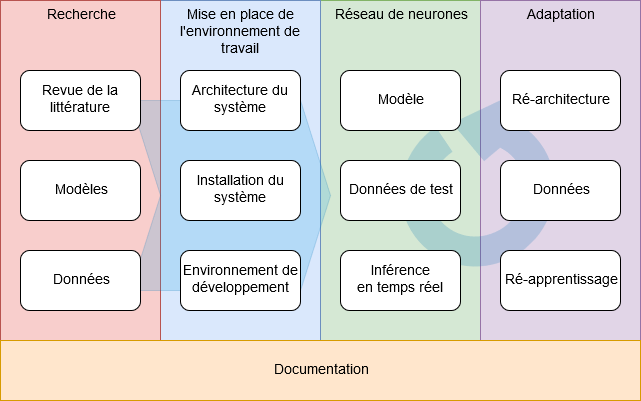
\includegraphics[width=1.0\textwidth]{methodologie}
    \caption{Organigrame de la méthodologie}
    \label{fig:methodologie1}
\end{figure}
\par L'objectif principal de l'essai est de déterminer la capacité et les limites du nano-ordinateur d'inférer en temps réel des modèles de réseau de neurones à convolution entier pour la segmentation sémantique de vidéos. La stratégie qui sera appliquée sera de tester avec divers modèles et divers niveaux de qualité vidéos, en espérant trouver le compromis qui répond le mieux à cet objectif.
\begin{enumerate}
   \item \label{metho:testbaseinférence} Afin de s'assurer du bon fonctionnement du nano-ordinateur et d'avoir des résultats de référence propre à notre environnement, l'inférence sera testée avec des modèles existants et pré-entrainés pour la segmentation sémantique, avec les images et les vidéos provenant des références, et dont les caractéristiques et les résultats sont disponibles. 
   \item \label{metho:testbaseinférencesite} En espérant que les tests de l'étape \#\ref{metho:testbaseinférence} précédente donnent les résultats documentés dans les articles de références, ils seront repris avec les mêmes modèles, mais avec les images et les vidéos du site d'étude possédant la meilleure qualité acquise (1080p/i, 30FPS). Les données sources (images et vidéos) devront subir certains prétraitements à ce effet, afin de répondre aux requis des modèles.
   \item \label{metho:testdevinférencesite} Selon les résultats de l'étape \#\ref{metho:testbaseinférencesite}, les tests se concentreront sur l'inférence avec des vidéos, en réduisant progressivement la résolution (760p/i, 576p/i, 480p/i, 360p/i) et le nombre d'images par seconde (20FPS, 10FSP, 1FPS).
   \item Les étapes intermédiaires de l'étape \#\ref{metho:testdevinférencesite} précédente seront de 1) valider les résultats de l'inférence avec des images avant de tester avec les vidéos, et 2) évaluer si les modèles de réseaux de neurones à convolution entiers doivent et/ou peuvent être adaptés facilement, en tenant compte de l'échéancier de l'essai, et ce afin de répondre à l'objectif principal.
\end{enumerate}
\par L'accès aux connaissances et à l'expérience de mon directeur de projet dans le domaine de l'apprentissage profond, ainsi que l'adhésion au "Deep Learning Institute" offerte par NVIDIA, sont les soutiens à ma disposition  pour arriver à compléter les objectifs de cet essai avec succès, et a trouver des solutions de contournement aux problèmes qui seront rencontrés.
\par À noter que l'acquisition des données du site d'étude se fera par l'intermédiaire d'une autre partie. La présentation du matériel et de la méthode d'acquisition des vidéos et des images terrain est donc exclue de cet essai.

\vspace{1\baselineskip}
\par 